\documentclass[twocolumn]{IEEEtran}
\usepackage[utf8x]{inputenc}
\usepackage{amssymb,amsfonts}
\usepackage[tbtags]{amsmath}
\usepackage{graphicx}
\usepackage{cite}
\usepackage{slashbox}
\usepackage{pict2e}
\usepackage{float}
\usepackage[all]{xy}
\usepackage{graphics,graphicx,color,colortbl}
\usepackage{times}
\usepackage{subfigure}
\usepackage{wrapfig}
\usepackage{multicol}
\usepackage{cite}
\usepackage{url}
\usepackage[tbtags]{amsmath}
\usepackage{amsmath,amssymb,amsfonts,amsbsy}
\usepackage{bm}
\usepackage{algorithm}
\usepackage{algorithmic}
\usepackage[centerlast, small]{caption}
\usepackage[colorlinks=true, citecolor=blue, linkcolor=blue, urlcolor=blue,
breaklinks=true]{hyperref}

\begin{document}
\title{Respuesta estacionaria de circuitos estimulados con $AC$}
\author{José Fabio Lozano Ovalle Código: $222982$\\
	Wilson Orlando Macias Fuquen Código: $223101$\\
	David Ricardo Martínez Hernández Código: $261931$}
\maketitle
\markboth{Universidad Nacional de Colombia}{}
\floatname{algorithm}{Algoritmo}

\begin{abstract}
Se construirán circuitos $RC$, $RL$ y $RLC$ alimentados por una señal sinusoidal y se analizara su respuesta en estado estable. Utilizando el osciloscopio y el método de las figuras de Lissajous se obtendrá  el ángulo de fase entre la tensión y la corriente en estos circuitos. También se construirán diagramas fasoriales para cada circuito y se verificara la variación del ángulo entre la tensión y el voltaje para diferentes frecuencias.
\end{abstract}

\begin{keywords}
Admitancias, Ángulo, Fase, Fasores, Frecuencia, Impedancias, Lissajous, Números Complejos, Parte Imaginaria, Parte Real, Periodo, Sinusoide.
\end{keywords}

\section{Objetivos}
\begin{itemize}
 \item Aprender a utilizar el osciloscopio para hallar figuras de Lissajous.
 \item Utilizar el método de figuras de Lissajous para determinar el ángulo entre tensión y corriente en circuitos $RL$, $RC$ y $RLC$.
 \item Utilizar la teoría fasorial para resolver circuitos alimentados por fuentes sinusoidales en estado estable.
 \item Obtener los diagramas fasoriales de cada circuito, y por medio de estos determinar ángulos de fase entre tensión y corriente.
\end{itemize}

\section{Marco Teórico}
\noindent
La respuesta de un circuito lineal se compone  de dos estados: La respuesta \textit{natural} y la respuesta \textit{forzada}.\\
La primera es la respuesta transitoria o respuesta de corto estado depende del cambio repentino a la que es sometido el elemento, la segunda es la respuesta de estado permanente de un circuito a cualquier fuente independiente presente.\\
Un \textbf{sinusoide} es una señal que tiene la forma de una función seno o coseno\footnote{Texto tomado de \cite{sadiku}, Página 354}.\\
Una corriente sinusoidal Hace referencia como una cualquier \textit{Corriente alterna (ac)}.

\subsection{Sinusoides}
\noindent
Considere un voltaje sinusoidal
\begin{equation}
 v(t) = V_{m} sin \omega t
\label{ecu1}
\end{equation}
\noindent
donde\\
$V_m = $es la \textit{amplitud} de el sinusoide\\
$\omega = $es la \textit{frecuencia angular}\\
$\omega t = $es el \textit{argumento} del sinusoide\\\\
La Fig. \ref{figa} es un sinusoide en función de su argumento y la Fig. \ref{figb} como una función del tiempo.
\begin{figure}[H]
  \centering
    \subfigure[Sinusoide en función de su argumento]{\label{figa}
      \fbox{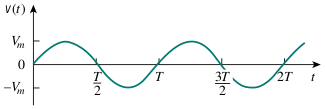
\includegraphics[scale=0.5]{sint.png}}}
  \hspace{2cm}
    \subfigure[Sinusoide en función del tiempo]{\label{figb}
      \fbox{\includegraphics[scale=0.5]{sinT.png}}}
  \caption{Funciones sinusoides (Imágenes tomadas de \cite{sadiku}, Página 355)}
    \label{fig1}
\end{figure}
\noindent
Es claro que el sinusoide se repite cada $T$ segundos, es decir $T$ es el \textit{periodo} de el sinusoide. Para las dos figuras el periodo es $\omega T = 2 \pi$
\begin{equation}
 T= \frac{2 \pi}{\omega}
\label{ecu2}
\end{equation}
\noindent
Si $v(t)$ se repite cada $T$ segundos, reemplazando $t$ por $t + T$ en la ecu. (\ref{ecu1}) se obtiene
\begin{equation}
 v(t+T) = V_{m} sin \omega (t + T) = V_{m} sin \omega (t + \frac{2 \pi}{\omega})
\label{ecu3}
\end{equation}
\begin{equation}
 v(t+T) = V_{m} sin (\omega t + 2 \pi) = V_{m} sin \omega t = v(t)
\label{ecu4}
\end{equation}
\noindent
entonces
\begin{equation}
 v(t+T) = v(t)
\label{ecu5}
\end{equation}
\noindent
Un \textbf{función periódica} es una función que satisface $f(t) = f(t + nT)$, para todo $t$ y todo $n$ entero\footnote{Texto tomado de \cite{sadiku}, Página 355}.\\
El periodo  $T$ de una función periódica es el tiempo de un ciclo completo. El reciproco de esta cantidad es el número de ciclos por segundo, conocida como la \textit{frecuencia cíclica} de el sinusoide.
\begin{equation}
 f = \frac{1}{T}
\label{ecu6}
\end{equation}
\noindent
Para las ecuaciones ecu. (\ref{ecu2}) y la ecu. (\ref{ecu6}) es claro que
\begin{equation}
 \omega = 2 \pi f
\label{ecu7}
\end{equation}
\noindent
Donde $\omega$ esta en radianes por segundo ($rad/s$), $f$ es en hertz ($Hz$).\\
\begin{equation}
 v(t) = V_{m} sin (\omega t + \phi)
\label{ecu8}
\end{equation}
\noindent
donde $(\omega t + \phi)$ es el argumento y $\phi$ es la \textit{fase}.

\subsection{Fasores}
\noindent
Un \textbf{fasor} es un número complejo que representa la amplitud y la fase de un sinusoide\footnote{Texto tomado de \cite{sadiku}, Página 359}.\\
Los fasores provienen de el análisis de circuitos lineales excitados por fuentes sinusoidales. Un número complejo $z$ puede ser escrito en su forma rectangular como 
\begin{equation}
 z = x + jy
\label{ecu9}
\end{equation}
\noindent
donde $j = \sqrt{-1}$; $x$ es la parte real de $z$; $y$ es la parte imaginaria de $z$.\\
El número complejo $z$ también puede escribirse de forma polar o exponencial como
\begin{equation}
 z = r\angle \phi  = r{e^{j\pi }}
\label{ecu10}
\end{equation}
\noindent
donde $r$ es la magnitud de $z$, y $\phi$ es la fase de $z$, se puede representar de tres maneras
\begin{equation}
 z = x+ jy
\label{ecu11}
\end{equation}
\begin{equation}
 z = r \angle \phi
\label{ecu12}
\end{equation}
\begin{equation}
 z = r{e^{j\phi }}
\label{cu13}
\end{equation}
\noindent
Las relaciones entre la forma rectangular y la forma polar mostrados en la Fig. \ref{fig2}
\begin{figure}[H]
	\centering
		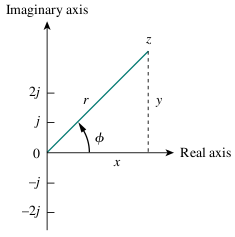
\includegraphics[scale=0.45]{reppolar.png}
	\caption{Representación de un número complejo $z = x +jy = r \angle \phi$ (Imagen tomada de  \cite{sadiku}, Página 360)}
	\label{fig2}
\end{figure}
\noindent
donde el eje $x$ representa la parte real y el eje $y$ representa la parte imaginaria del número complejo. En función de $x$ y $y$, se puede representar $r$ y $\phi$ como
\begin{equation}
 r = \sqrt{x^2 + y^2}, \ \ \ \ \ \phi = {\tan ^{ - 1}}\frac{y}{x} 
\label{ecu14}
\end{equation}
\noindent
Por otra parte si se conoce $r$ y $\phi$, se puede obtener $x$ y $y$ como
\begin{equation}
 x = r cos \phi \ \ \ \ \ \ y = r sin \phi
\label{ecu15}
\end{equation}
\noindent
$z$ se puede escribir como
\begin{equation}
 z = x + jy = r \angle \phi = r(cos \phi + j sin \phi)
\label{ecu16}
\end{equation}
\noindent
Las operaciones básicas se realizan de la siguiente manera:\\
\textbf{Adición:}
\begin{equation}
 z_1 + z_2 = (x_1 + x_2)+ j(y_1 + y_2)
\label{ecu17}
\end{equation}
\noindent
\textbf{Substracción:}
\begin{equation}
 z_1 - z_2 = (x_1 - x_2)+ j(y_1 - y_2)
\label{ecu18}
\end{equation}
\noindent
\textbf{Multiplicación:}
\begin{equation}
 z_1 z_2 = r_1 r_2 \angle (\phi _1 + \phi _2)
\label{ecu19}
\end{equation}
\noindent
\textbf{División:}
\begin{equation}
 \frac{z_1}{z_2} = \frac{r_1}{r_2} \angle (\phi _1 - \phi _2)
\label{ecu20}
\end{equation}
\noindent
\textbf{Reciproco:}
\begin{equation}
 \frac{1}{z} = \frac{1}{r} \angle -\phi
\label{ecu21}
\end{equation}
\noindent
\textbf{Raíz Cuadrada:}
\begin{equation}
 \sqrt{z} = \sqrt{r} \angle (\phi /2)
\label{ecu22}
\end{equation}
\noindent
\textbf{Conjugado complejo:}
\begin{equation}
 z^{*} = x -jy = r \angle - \phi = r{e^{-j\phi }}
\label{ecu23}
\end{equation}
\begin{table}[H]
	\centering
\begin{tabular}[c]{|c|c|} \hline
Representación en el tiempo & Representación en fasores \\ \hline
$V_m cos (\omega t + \phi)$ & $V_m \angle \phi$ \\
$V_m sin (\omega t + \phi)$ & $V_m \angle (\phi- 90°)$ \\
$I_m cos (\omega t + \phi)$ & $I_m \angle \phi$ \\
$I_m sin (\omega t + \phi)$ & $I_m \angle (\phi- 90°)$ \\ \hline
\end{tabular}
	\caption{Transformaciones de sinusoides a fasores (Tomado de \cite{sadiku}, Página 363)}
	\label{tab1}
\end{table}
\noindent
La \textbf{impedancia} $Z$ de un circuito es la relación entre la tensión  $V$ y la corriente $I$ de fasor, medida en Ohmios $(\Omega)$\footnote{Texto tomado de \cite{sadiku}, Página 370}.\\
La \textbf{admitancia} $Y$ es el reciproco de la impedancia medida en siemens $(S)$\footnote{Texto tomado de \cite{sadiku}, Página 371}.
\begin{table}[H]
	\centering
\begin{tabular}[c]{|c|c|c|} \hline
Elemento & Impedancia & Admitanica \\ \hline
$R$ & $Z = R$ & $Y = \frac{1}{R}$ \\
$L$ & $Z = j \omega L$ & $Y = \frac{1}{j \omega L}$ \\
$C$ & $Z = \frac{1}{j \omega C}$ & $Y = j \omega C$ \\ \hline
\end{tabular}
	\caption{Impedancias y Admitancias de elementos pasivos (Tomado de \cite{sadiku}, Página 363)}
	\label{tab2}
\end{table}
\noindent
Los teoremas para solucionar circuitos en fasores son los mismos y llevan el mismo procedimiento que los utilizados en circuitos $DC$, tomando el voltaje y la corriente en su forma fasorial, y la resistencia por una impedancia, la cual lleva una parte real y una parte imaginaria.

\subsection{Curvas de Lissajous}
\noindent
Las curvas de Lissajous son gráficas de ecuaciones paramétricas, correspondientes a la superposición de dos movimientos armónicos simples en direcciones perpendiculares,  estas gráficas fueron  investigadas por \textbf{Nathaniel Bowditch}, y posteriormente con mayores detalles por \textbf{Jules Antoine Lissajous}.\\
La característica principal de la figura es que, debido a su característica de representar dos ecuaciones paramétricas sinusoidales, esta gráfica es sensible a la relación de la frecuencia de las dos señales, la fase y la amplitud entre ellas, como se observa en la Fig. \ref{fig3}
\begin{figure}[H]
	\centering
		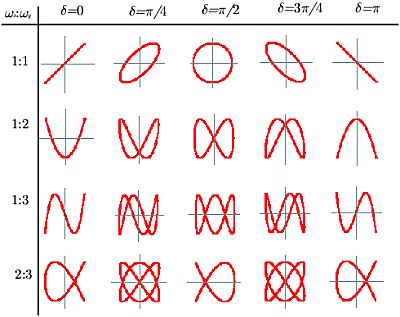
\includegraphics[scale=0.5]{lissa.png}
	\caption{Gráficas de Lissajous (Imagen tomada de \cite{page2})}
	\label{fig3}
\end{figure}

\section{Hipótesis}
En un circuito $RL$ la corriente en el inductor se encuentre 90 grados atrasada respecto a la tensión y la de la resistencia esta en fase con el voltaje.\\
En un circuito $RC$ la corriente en el capacitor se encuentre $90^\circ$ adelantada respecto a la tensión y la de la resistencia esta en fase con el voltaje.\\
Las curvas de Lissajous que se obtendrán para los circuitos $RL$ y $RC$ serán de la forma:
\begin{figure}[H]
	\centering
		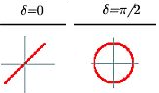
\includegraphics[scale=1]{fig1.png}
	\caption{Curvas que se obtendrán}
	\label{fig11}
\end{figure}

\section{Materiales}
\begin{itemize}
 \item Bobina
 \item Condensador
 \item Generador de Señales
 \item Multímetro
 \item Osciloscopio
 \item Resistencias
\end{itemize}

\section{Análisis y Resultados Teórico}
\noindent
Para esta práctica se implementarán tres circuitos los cuales  se muestran a continuación y sus cálculos correspondientes, además el diagrama fasorial. Para cada circuito se usara una fuente $AC$ con un $V_p=5\ V$  a una frecuencia $f = 1000\ Hz$.

\subsection{Circuito $RL$}
\noindent
Para el siguiente circuito se hace un análisis fesorial por el método de mallas
\begin{figure}[H]
	\centering
		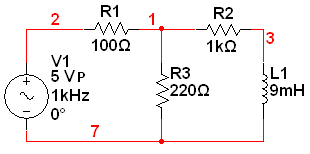
\includegraphics[scale=0.75]{circ1.png}
	\caption{Montaje del circuito $RL$}
	\label{fig4}
\end{figure}
\begin{equation}
 {Z_L} = j\omega L = j56.549
\label{ecu24}
\end{equation}
\begin{equation}
 5\angle 0^\circ  = {i_1}(100 + 220) - {i_2}(220)
\label{ecu25}
\end{equation}
\begin{equation}
 0 = {i_2}\left( {1000 + 220 + j56.549} \right) - {i_1}(220)
\label{ecu26}
\end{equation}
\noindent
Con la solución del sistema anterior se obtienen los siguientes datos:
\begin{table}[H]
	\centering
\begin{tabular}[c]{|c|c|c|} \hline
Elemento & Tensión $[V]$ & Corriente $[mA]$ \\ \hline
$R_1$ & $1.782 \angle -0.3748°$ & $17.83 \angle -0.3748°$ \\ \hline
$R_2$ & $3.2119 \angle -3.0288°$ & $3.2119 \angle -3.0288°$ \\ \hline
$R_3$ & $4.62836 \angle 0.14448°$ & $21.038 \angle 0.14448°$ \\ \hline
$L_1$ & $0.18163 \angle 86.971°$ & $3.2119 \angle -3.0288°$ \\ \hline
\end{tabular}
	\caption{Valores obtenidos teóricamente}
	\label{tab3}
\end{table}
\noindent
Luego se muestra el diagrama fasorial de la tensión y corriente en la inductancia, donde $V_L=Z_1$ y $I_L=Z_2$
\begin{figure}[H]
	\centering
		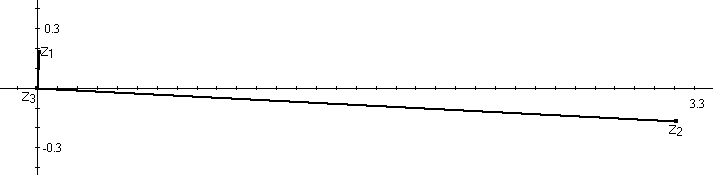
\includegraphics[scale=0.35]{fa1.png}
	\caption{Diagrama Fasorial circuito $RL$}
	\label{fig5}
\end{figure}

\subsection{CIRCUITO $RC$}
\noindent
Para este circuito se hace un análisis fasorial de por mallas.
\begin{figure}[H]
	\centering
		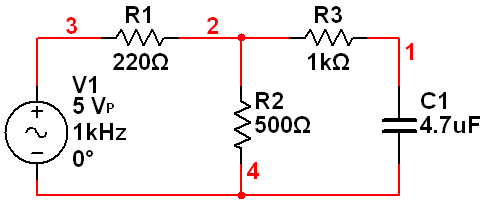
\includegraphics[scale=0.5]{circ2.png}
	\caption{Montaje del circuito $RL$}
	\label{fig6}
\end{figure}
\noindent
\begin{equation}
 Z_c = \frac{1}{{j\omega c}} =  - j33.863
\label{ecu27}
\end{equation}
\begin{equation}
 5\angle 0^\circ  = {i_1}(220 + 500) - {i_2}(500)
\label{ecu28}
\end{equation}
\begin{equation}
 0 = {i_2}\left( {1000 + 500 - j33.863} \right) - {i_1}(500)
\label{ecu29}
\end{equation}
\noindent
Al solucionar el sistema de ecuaciones se tiene los siguientes datos:
\begin{table}[H]
	\centering
\begin{tabular}[c]{|c|c|c|} \hline
Elemento & Tensión $[V]$ & Corriente $[mA]$ \\ \hline
$R_1$ & $1.987634 \angle -0.38929°$ & $9.0347 \angle -0.38929°$ \\ \hline
$R_2$ & $6.022 \angle -0.12854°$ & $12.044 \angle -0.12854°$ \\ \hline
$R_3$ & $3.30107 \angle 1.6826°$ & $3.30107 \angle 1.62826°$ \\ \hline
$C_1$ & $0.30594 \angle -89.611°$ & $9.0347 \angle 0.38929°$ \\ \hline
\end{tabular}
	\caption{Valores obtenidos teóricamente}
	\label{tab4}
\end{table}
\noindent
A continuación se tiene la gráfica fasorial de la corriente y la tensión en el capacitor, donde $V_C=Z_1$ y $I_C=Z_2$.
\begin{figure}[H]
	\centering
		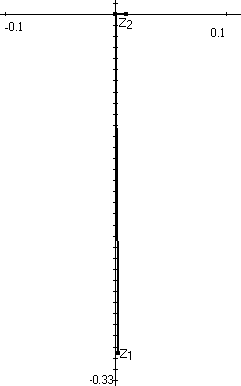
\includegraphics[scale=0.45]{fa2.png}
	\caption{Diagrama Fasorial circuito $RC$}
	\label{fig7}
\end{figure}

\subsection{Circuito $RLC$}
\noindent
Para el siguiente circuito se hace un análisis fasorial por el método de mallas para observar el comportamiento del circuito en estado estacionario.
\begin{figure}[H]
	\centering
		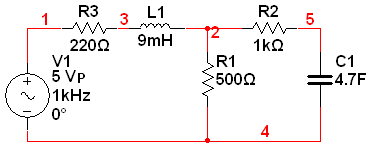
\includegraphics[scale=0.75]{circ3.png}
	\caption{Montaje del circuito $RLC$}
	\label{fig8}
\end{figure}
\begin{equation}
 Z_C = \frac{1}{{j\omega c}} =  - j33.863
\label{ecu30}
\end{equation}
\begin{equation}
 {Z_L} = j\omega L = j56.549
\label{ecu31}
\end{equation}
\begin{equation}
 5\angle 0^\circ  = {i_1}(220 + 500 + j56.549) - {i_2}(500)
\label{ecu32}
\end{equation}
\begin{equation}
 0=i_2 (1000+500-j33.863)-i_1 (500)
\label{ecu33}
\end{equation}
\noindent
A partir de la solución del sistema anterior se obtienen los siguientes datos:
\begin{table}[H]
	\centering
\begin{tabular}[c]{|c|c|c|} \hline
Elemento & Tensión $[V]$ & Corriente $[mA]$ \\ \hline
$R_1$ & $2.999 \angle -6.0938 ^\circ$ & $5.9979 \angle -6.0938^\circ$ \\ \hline
$R_2$ & $2.9972 \angle -4.1555^\circ$ & $2.9972 \angle -4.1555^\circ$ \\ \hline
$R_3$ & $1.9787 \angle -5.448^\circ$ & $8.994 \angle -5.448^\circ$ \\ \hline
$C_1$ & $0.10149 \angle -94.156^\circ$ & $0.0029978 \angle 4.1555^\circ$ \\ \hline
$C_1$ & $0.5089 \angle 84.552^\circ$ & $8.994 \angle -5.448^\circ$ \\ \hline
\end{tabular}
	\caption{Valores obtenidos teóricamente}
	\label{tab5}
\end{table}
\noindent
Para este circuito se tienen los diagramas fasoriales en $C_1$ y $L_1$.\\
Para este gráfico $V_C=Z_1$ y $I_C=Z_2$:
\begin{figure}[H]
	\centering
		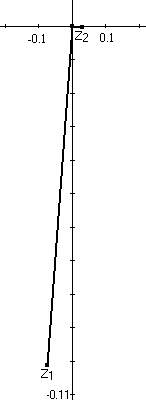
\includegraphics[scale=0.45]{fa3.png}
	\caption{Diagrama Fasorial circuito $RCL$}
	\label{fig9}
\end{figure}
\noindent
Para el siguiente diagrama se tiene que $V_L=Z_1$ y $I_L=Z_2$. 
\begin{figure}[H]
	\centering
		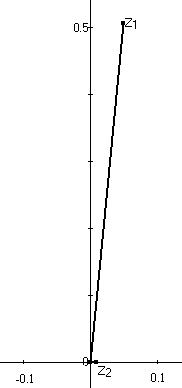
\includegraphics[scale=0.45]{fa4.png}
	\caption{Diagrama Fasorial circuito $RCL$}
	\label{fig10}
\end{figure}

\section{Preguntas}
\begin{enumerate}
 \item ¿Como es el ángulo de fase entre la tensión y la corriente de cada uno de los circuitos $RL$, $RC$ y $RLC$?\\
Elegimos una amplitud de tensión de la fuente de $V_M$ y un ángulo de fase de cero grados.\\
Para un circuito $RL$ el ángulo de fase de la corriente dependerá de la relación entre la tensión y la impedancia y como elegimos el ángulo de la fuente de tensión en cero grados, la corriente tendrá un ángulo de fase dependiente de la impedancia:
\begin{equation}
 \phi = -tan^{-1} \frac{\omega L}{R}
\label{ecu34}
\end{equation}
Utilizando la misma consideración para la fuente, en un circuito RC la corriente tendrá un ángulo de fase:
\begin{equation}
 \phi  =  - ta{n^{ - 1}}\frac{1}{{R\omega C}}
\label{ecu35}
\end{equation}
Para un circuito $RLC$ en serie tenemos que la corriente tendrá un ángulo de fase:
\begin{equation}
 \phi  =  - ta{n^{ - 1}}\frac{{\omega L - \frac{1}{{\omega C}}}}{R}
\label{ecu36}
\end{equation}

 \item ¿El ángulo de fase entre la tensión y la corriente en circuitos $RL$, $RC$ y $RLC$ varía con respecto a la frecuencia?\\
Si varía puesto que la impedancia del inductor y del condensador dependen directamente de la frecuencia:
\begin{equation}
 {Z_L} = j\omega L \ \ \ \ \ \ {Z_C} = \frac{1}{{j\omega C}}
\label{ecu37}
\end{equation}
\noindent
$\omega=2 \pi f$ siendo $f$ la frecuencia.

 \item ¿Que diferencias hay entre los ángulos medidos usando las figuras de Lissajous y usando la visualización en función del tiempo de osciloscopio?\\
No debería haber ninguna, pero eso se responderá en la práctica.
 \item ¿Que utilidad tiene el uso de los fasores en el análisis de circuitos en contraposición con los análisis realizados en las prácticas anteriores?\\
Las tensiones, corrientes e impedancias en un circuito de corriente alterna se pueden representar como vectores en el plano complejo, la notación fasorial toma los valores de magnitud y ángulo de dichos vectores y esto permite que los cálculos sean más cortos.
 \item ¿Coinciden las magnitudes y ángulos de fase obtenidos experimentalmente con los valores teóricos?\\
Esta pregunta se responderá con los resultados de la práctica.
\end{enumerate}

\bibliographystyle{ieeetran}
\begin{thebibliography}{99}
\bibitem{sadiku} Alexander, Charles K. \&  Sadiku, Matthew N.O.
{\em ```Fundamentals of Electric Circuits"'}.
McGRAW-HILL, ISE Editions, 1999.

\bibitem{dorf} Dorf  \& Svoboda.
{\em ```Circuitos Eléctricos"'}.
Alfaomega, Sexta Edición, 2006.

\bibitem{hayt} Hayt, William H. Jr., Kemmerly, Jack E. \& Durbin, Steven M.
{\em ```Análisis de circuitos en ingeniería"'}.
McGRAW-HILL, Séptima Edición, 2007.

\bibitem{nahvi} Nahvi, Mahmood \& Edminister, Joseph A.
{\em ```Theory and Problems of Electric Circuits"'}.
McGRAW-HILL, Fourth Edition, 2003.

\bibitem{page1} \url{http://es.wikipedia.org/wiki/Curva_de_Lissajous}. Visitada el 18 de septiembre de 2011.

\bibitem{page2} \url{http://www.chochitopelao.com/las-curvas-de-lissajous/}.
Visitada el 18 de septiembre de 2011.

\end{thebibliography}
\end{document}